%%%%%%%%%%%%%%%%%%%%%%%%%%%%%%%%%%%%%%%%%
% Beamer Presentation
% LaTeX Template
% Version 1.0 (10/11/12)
%
% This template has been downloaded from:
% http://www.LaTeXTemplates.com
%
% License:
% CC BY-NC-SA 3.0 (http://creativecommons.org/licenses/by-nc-sa/3.0/)
%
%%%%%%%%%%%%%%%%%%%%%%%%%%%%%%%%%%%%%%%%%

%----------------------------------------------------------------------------------------
%	PACKAGES AND THEMES
%----------------------------------------------------------------------------------------

\documentclass{beamer}

\mode<presentation> {

% The Beamer class comes with a number of default slide themes
% which change the colors and layouts of slides. Below this is a list
% of all the themes, uncomment each in turn to see what they look like.

%\usetheme{default}
%\usetheme{AnnArbor}
%\usetheme{Antibes}
%\usetheme{Bergen}
%\usetheme{Berkeley}
%\usetheme{Berlin}
%\usetheme{Boadilla}
%\usetheme{CambridgeUS}
%\usetheme{Copenhagen}
%\usetheme{Darmstadt}
%\usetheme{Dresden}
%\usetheme{Frankfurt}
%\usetheme{Goettingen}
%\usetheme{Hannover}
%\usetheme{Ilmenau}
%\usetheme{JuanLesPins}
%\usetheme{Luebeck}
\usetheme{Madrid}
%\usetheme{Malmoe}
%\usetheme{Marburg}
%\usetheme{Montpellier}
%\usetheme{PaloAlto}
%\usetheme{Pittsburgh}
%\usetheme{Rochester}
%\usetheme{Singapore}
%\usetheme{Szeged}
%\usetheme{Warsaw}

% As well as themes, the Beamer class has a number of color themes
% for any slide theme. Uncomment each of these in turn to see how it
% changes the colors of your current slide theme.

%\usecolortheme{albatross}
%\usecolortheme{beaver}
%\usecolortheme{beetle}
%\usecolortheme{crane}
%\usecolortheme{dolphin}
%\usecolortheme{dove}
%\usecolortheme{fly}
%\usecolortheme{lily}
%\usecolortheme{orchid}
%\usecolortheme{rose}
%\usecolortheme{seagull}
%\usecolortheme{seahorse}
%\usecolortheme{whale}
%\usecolortheme{wolverine}

%\setbeamertemplate{footline} % To remove the footer line in all slides uncomment this line
%\setbeamertemplate{footline}[page number] % To replace the footer line in all slides with a simple slide count uncomment this line

%\setbeamertemplate{navigation symbols}{} % To remove the navigation symbols from the bottom of all slides uncomment this line
}
	
\usepackage{graphicx} % Allows including images
\usepackage{booktabs} % Allows the use of \toprule, \midrule and \bottomrule in tables

%\usepackage{float}
%\usepackage{subfigure}
%\usepackage{subfig}
%\usepackage{lipsum}
%\usepackage{caption}
%\usepackage{verbatim}

\usepackage{biblatex}



%----------------------------------------------------------------------------------------
%	TITLE PAGE
%----------------------------------------------------------------------------------------

\title[Advanced Image Analysis]{Bilateral Filters} % The short title appears at the bottom of every slide, the full title is only on the title page

\author{Emre Ozan ALKAN} % Your name
\institute[MSCV] % Your institution as it will appear on the bottom of every slide, may be shorthand to save space
{
University of Burgundy \\ % Your institution for the title page
\medskip
\textit{emreozanalkan@gmail.com} % Your email address
}
\date{\today} % Date, can be changed to a custom date

\begin{document}

\begin{frame}
\titlepage % Print the title page as the first slide
\end{frame}

\begin{frame}
\frametitle{Overview} % Table of contents slide, comment this block out to remove it
\tableofcontents % Throughout your presentation, if you choose to use \section{} and \subsection{} commands, these will automatically be printed on this slide as an overview of your presentation
\end{frame}

%----------------------------------------------------------------------------------------
%	PRESENTATION SLIDES
%----------------------------------------------------------------------------------------

\section{Introduction}

\begin{frame}
\frametitle{Introduction}
\begin{itemize}
	\item Fundemental process in CV
	\pause
	\item Aim: reduce noise
	\pause
	\item Many filters: Mean, Median, Gaussian
	\pause
	\item Pourquoi Bilateral Filter ?
\end{itemize}
\end{frame}

\section{Problems in Filtering}

\begin{frame}
\frametitle{Problems in Filtering}
\begin{itemize}
	\item Gaussian filtering - low pass
	\pause
	\item Details lost
	\pause
	\item Blurred edges
\end{itemize}
\end{frame}

\section{Bilateral Filtering}
% DIVIDE THIS TO 2 PAGES
\begin{frame}
\frametitle{Bilateral Filtering}
\begin{itemize}
	\item Smooths images while preserving
edges
	\pause
	\item Nonlinear combination of nearby
image values
	\pause
	\item Geometric closeness
	\pause
	\item Photometric similarity
	\pause
	\item Prefers near values to distant values

\end{itemize}
\end{frame}

\begin{frame}
\frametitle{Bilateral Filtering}
\begin{itemize}
	\item Noniterative, local, and simple
	\pause
	\item CIE-Lab color space
	\pause
	\item No phantom colors

\end{itemize}
\end{frame}

\section{Algorithm}

\begin{frame}
\frametitle{Algorithm}
The filter can be defined as:
\begin{equation} \label{eq:filter}
 I^\text{filtered}(x) = \frac{1}{W_p} \sum_{x_i \in \Omega} I(x_i)f_r(\|I(x_i)-I(x)\|)g_s(\|x_i-x\|)
\end{equation}

where the normalization $W_{p}$ is defined as:
\begin{equation} \label{eq:weight}
W_p = \sum_{x_i \in \Omega}{f_r(\|I(x_i)-I(x)\|)g_s(\|x_i-x\|)}
\end{equation}

$x$ are coordinates of the current pixel to be filtered;\\
$\Omega $  is the window centered in $x$\\
$f_{r}$ is the range kernel for smoothing differences in intensities\\
$g_{s}$ is the spatial kernel for smoothing differences in coordinates

\end{frame}

\begin{frame}[fragile]
\frametitle{Algorithm}

\fontsize{7pt}{9pt}\selectfont
%\verbatiminput{bilateralFiltering.m}
\begin{verbatim}
function outputImage = bilateralFilter(inputImage, w, sigma_d, sigma_r)
% Pre-compute Gaussian distance weights.
[X,Y] = meshgrid(-w : w, -w : w);
G = exp(-(X.^2 + Y.^2) / (2 * sigma_d ^ 2));
% Apply bilateral filter.
dim = size(inputImage);
outputImage = zeros(dim);
for i = 1:dim(1)
   for j = 1:dim(2)
         % Extract local region.
         iMin = max(i - w, 1);
         iMax = min(i + w, dim(1));
         jMin = max(j - w, 1);
         jMax = min(j + w,dim(2));
         I = A(iMin : iMax, jMin : jMax);
         % Compute Gaussian intensity weights.
         H = exp(-(I - A(i,j)).^2 / (2 * sigma_r ^ 2));
         % Calculate bilateral filter response.
         F = H .* G((iMin : iMax) -i + w + 1, (jMin : jMax) - j + w + 1);
         outputImage(i, j) = sum(F(:) .* I(:)) / sum(F(:));
   end
end
\end{verbatim}

\end{frame}

\begin{frame}
\frametitle{Algorithm}
\begin{figure}
%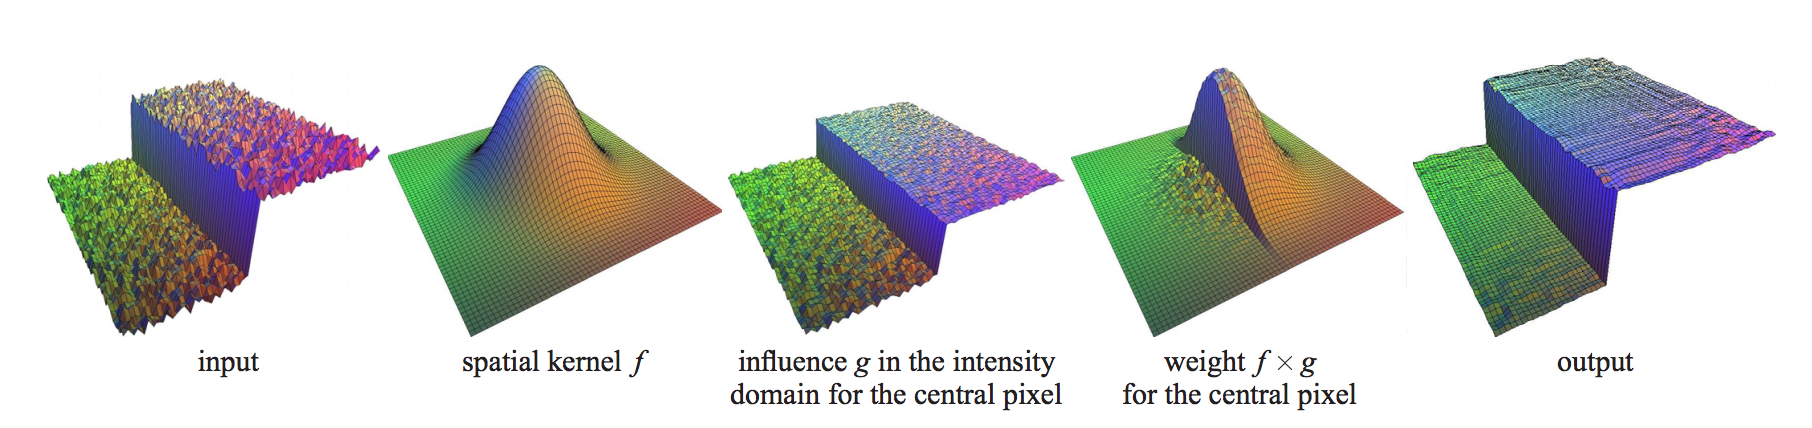
\includegraphics[scale=0.19]{Overall}
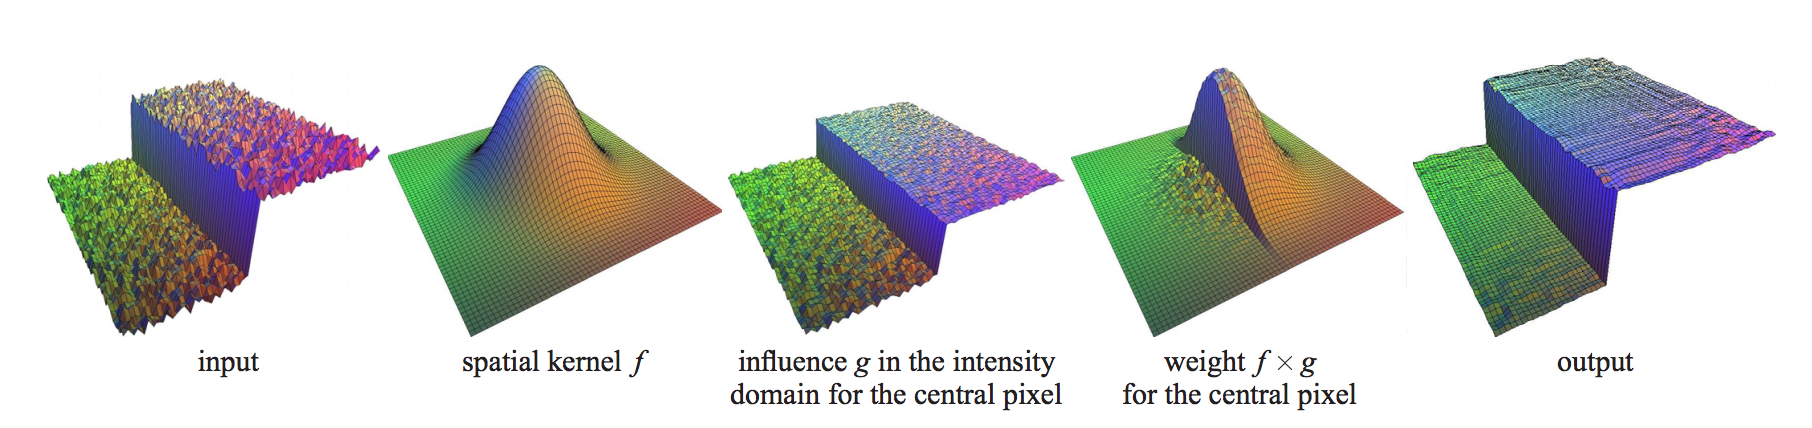
\includegraphics[width=1\linewidth]{Overall}
\caption{Overall}
\end{figure}
\end{frame}

\begin{frame}
\frametitle{Algorithm}
\begin{figure}
%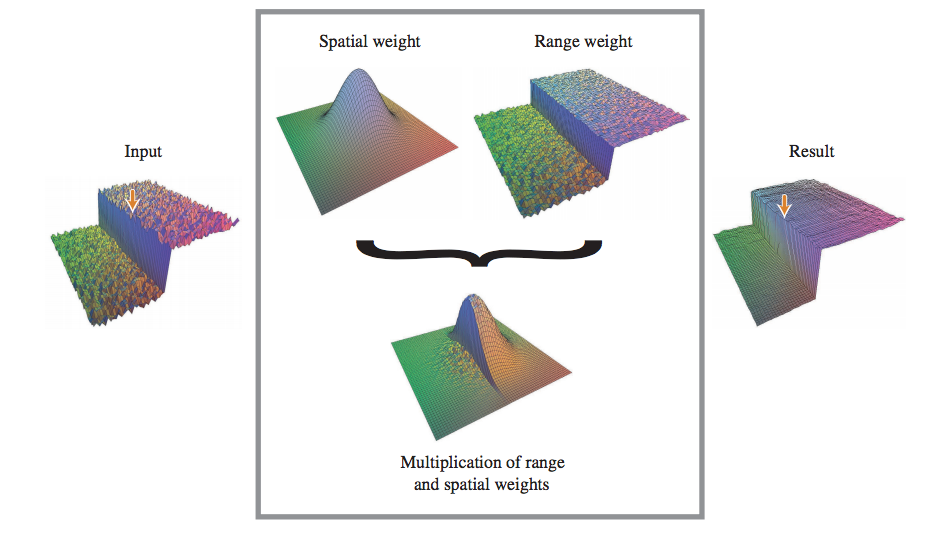
\includegraphics[scale=0.35]{OverallProcess}
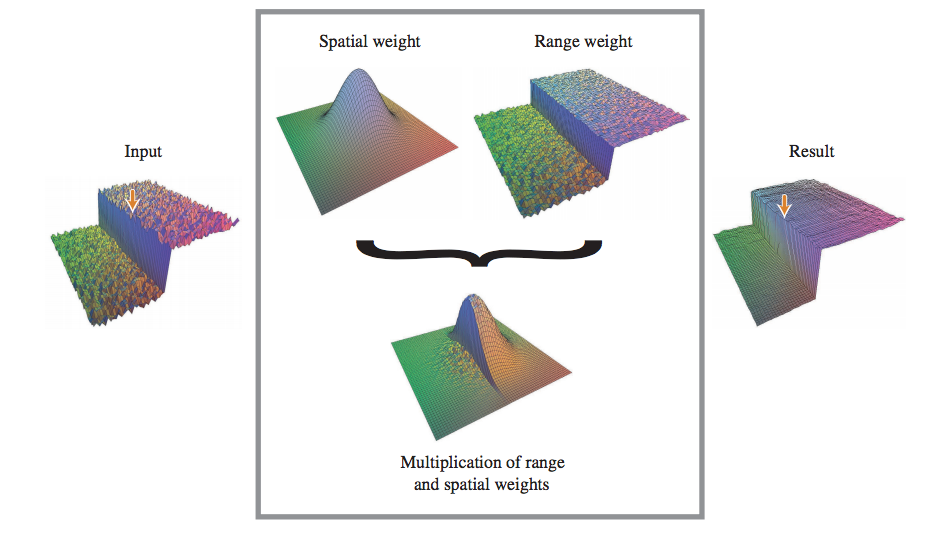
\includegraphics[width=1\linewidth]{OverallProcess}
\caption{Overall Process}
\end{figure}
\end{frame}

\section{Results}

\begin{frame}
\frametitle{Results}
\begin{figure}
%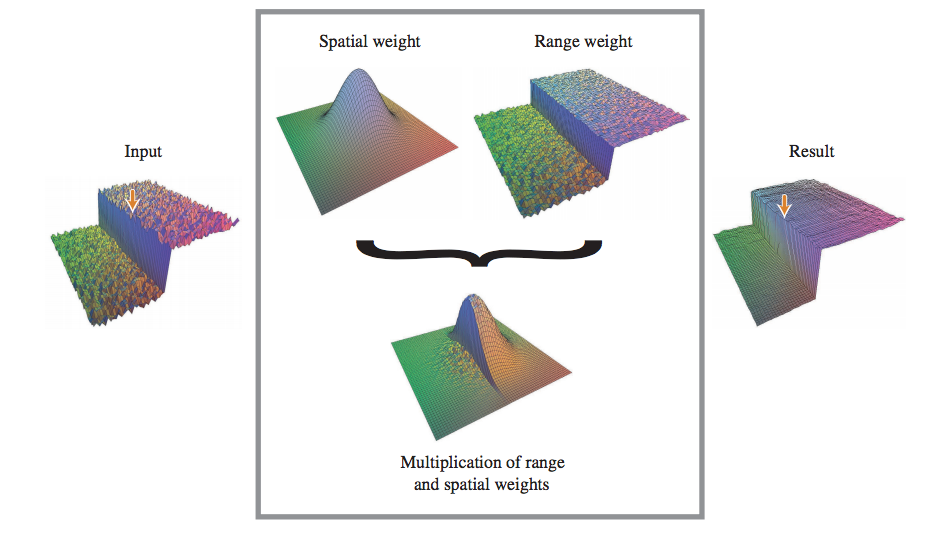
\includegraphics[scale=0.35]{OverallProcess}
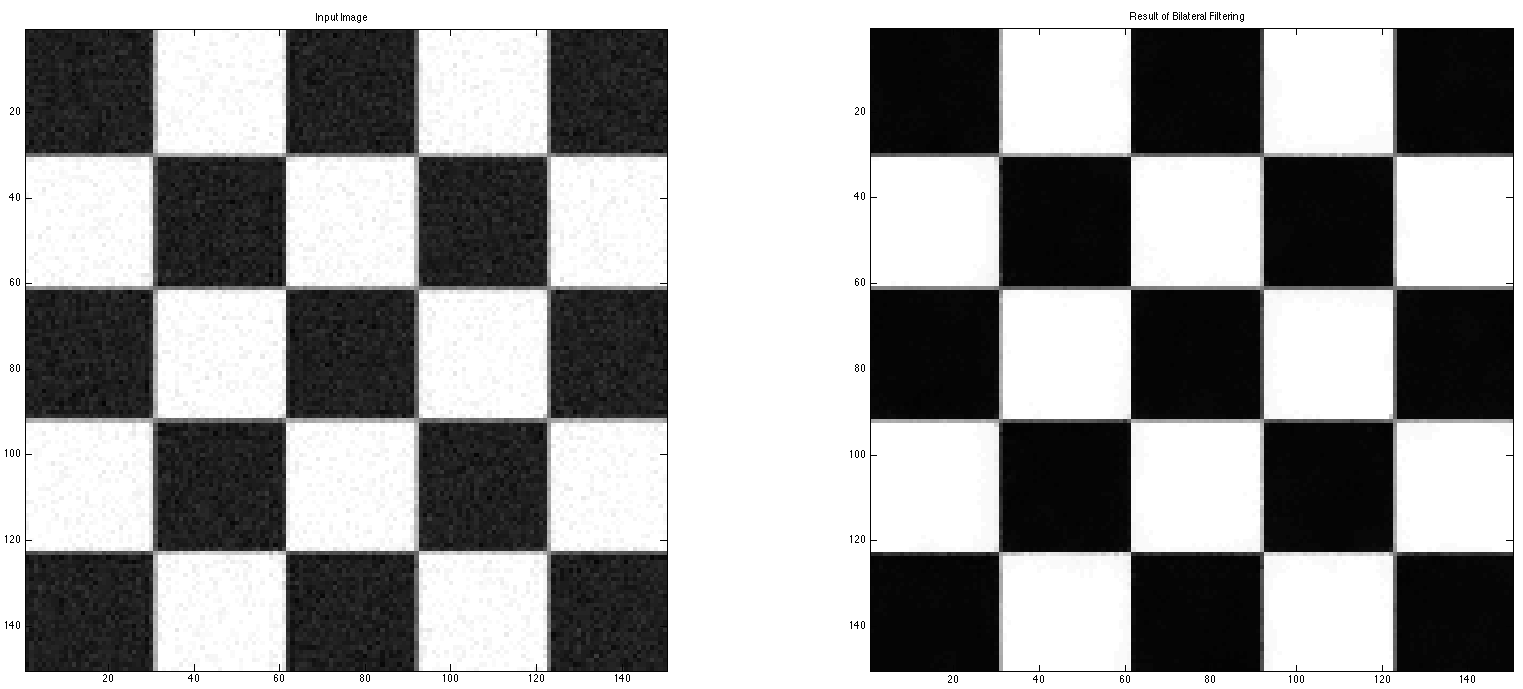
\includegraphics[width=1\linewidth]{syn1}
\caption{Denoising synthetic image}
\end{figure}
\end{frame}

\begin{frame}
\frametitle{Results}
\begin{figure}
%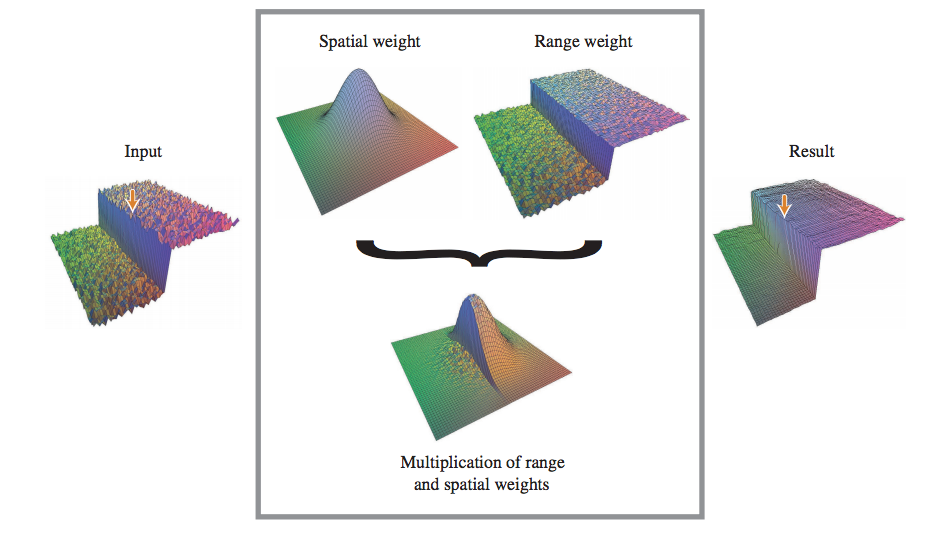
\includegraphics[scale=0.35]{OverallProcess}
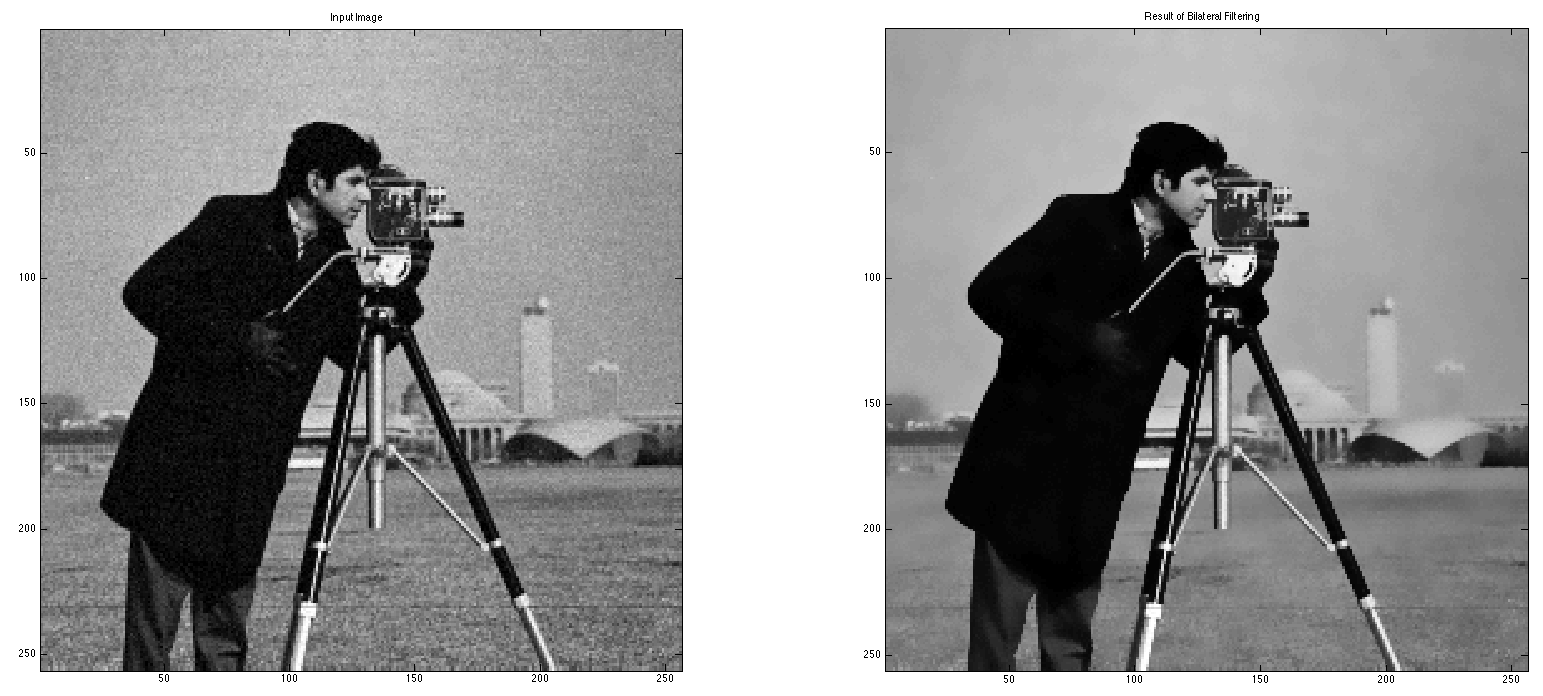
\includegraphics[width=1\linewidth]{bw1}
\caption{Denoising gray-scale image}
\end{figure}
\end{frame}

\begin{frame}
\frametitle{Results}
\begin{figure}
%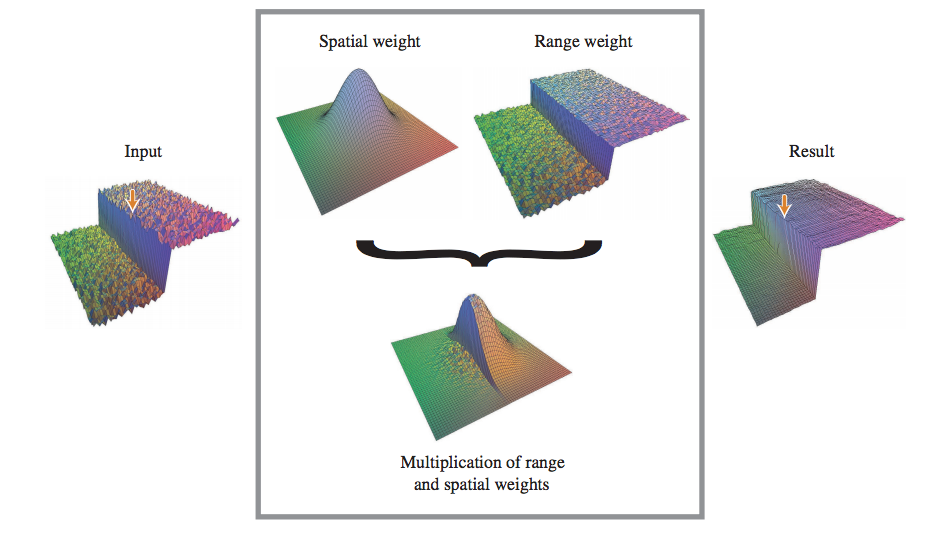
\includegraphics[scale=0.35]{OverallProcess}
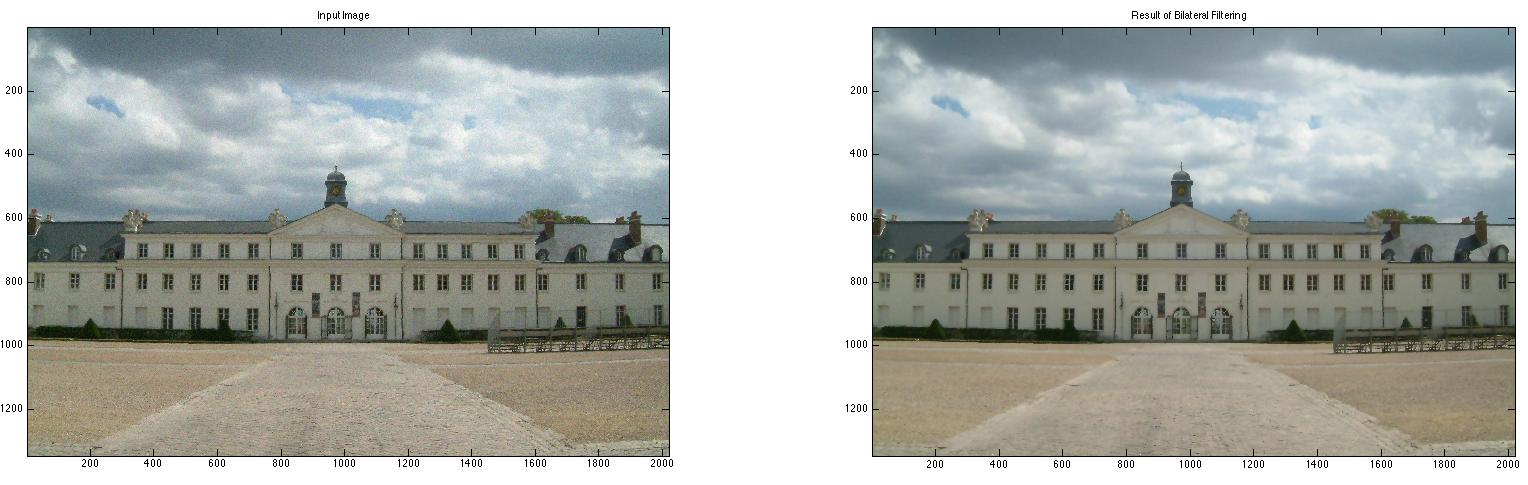
\includegraphics[width=1\linewidth]{color1.png}
\caption{Denoising color image}
\end{figure}
\end{frame}

\begin{frame}
\frametitle{Results}
\begin{figure}
\includegraphics[width=0.85\linewidth]{wineOnion}
\end{figure}
\end{frame}

\begin{frame}
\frametitle{Results}
\begin{figure}
   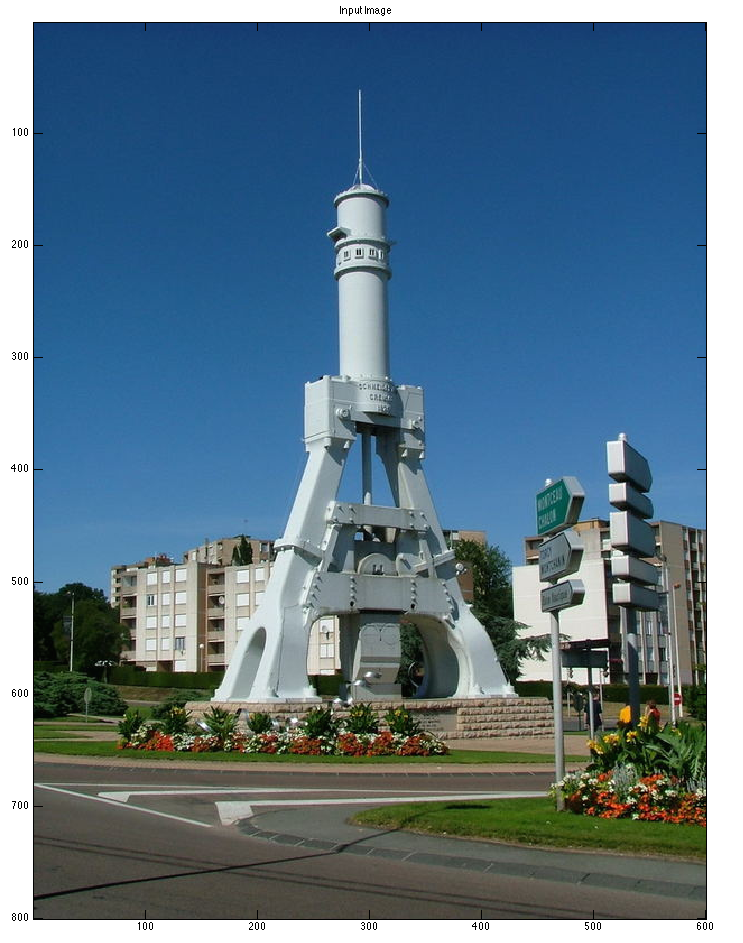
\includegraphics[width=0.47\linewidth]{e1}
   %\hfill
   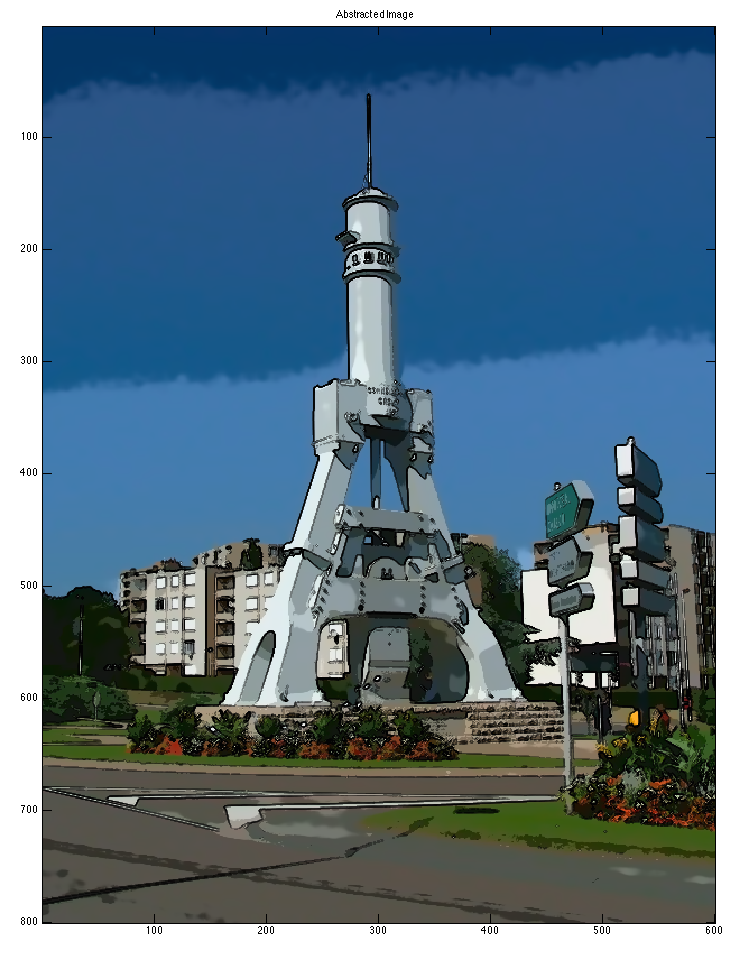
\includegraphics[width=0.47\linewidth]{ae1}
   \caption{Image Abstraction}
\end{figure}
\end{frame}

\begin{frame}
\frametitle{Results}
\begin{figure}
\includegraphics[width=0.9\linewidth]{catParams}
\caption{Cat Image: Range and Domain Parameters}
\end{figure}
\end{frame}

\begin{frame}
\frametitle{Results}
\begin{figure}
\includegraphics[width=0.99\linewidth]{houseParams}
\caption{House Image: Range and Domain Parameters}
\end{figure}
\end{frame}

\begin{frame}
\frametitle{Results}
\begin{block}{Parameters}
The bilateral filter is controlled by two parameters: $ \sigma_{s} $ and $ \sigma_{r} $.
\end{block}

\begin{block}{Range}
As the range parameter $ \sigma_{r} $ increases, the bilateral filter becomes closer to Gaussian blur
because the range Gaussian is flatter i.e., almost a constant over the intensity interval
covered by the image
\end{block}

\begin{block}{Domain}
Increasing the spatial parameter $ \sigma_{s} $ smooths larger features.
\end{block}
\end{frame}

\section{Applications}

\begin{frame}
\frametitle{Applications}
\begin{itemize}
	\item Denoising
	\pause
	\item Contrast reduction
	\pause
	\item Adobe Photoshop: surface blur tool
	\pause
	\item GIMP: Filters $\rightarrow$ Blur tools $\rightarrow$ Selective Gaussian Blur
	\pause
	\item 3D Fairing - Mesh smoothing
	\pause
	\item Cartoonizing applications
\end{itemize}
\end{frame}

\section{Limitations}
\begin{frame}
\frametitle{Limitations}
The basic bilateral filter introduce several types of image artifacts:
\pause
\begin{itemize}
	\item Staircase effect - image appearing like cartoons and contours
	\item Gradient reversal - introduction of false edges
\end{itemize}
\end{frame}
%The bilateral filter in its direct form can introduce several types of image artifacts:
%
%Staircase effect - intensity plateaus that lead to images appearing like cartoons [1]
%Gradient reversal - introduction of false edges in the image [2]
%There exist several extensions to the filter that deal with these artifacts. Alternative filters, like the guided filter [3], have also been proposed as an efficient alternative without these limitations.

\begin{frame}
\frametitle{Limitations}
\begin{figure}
%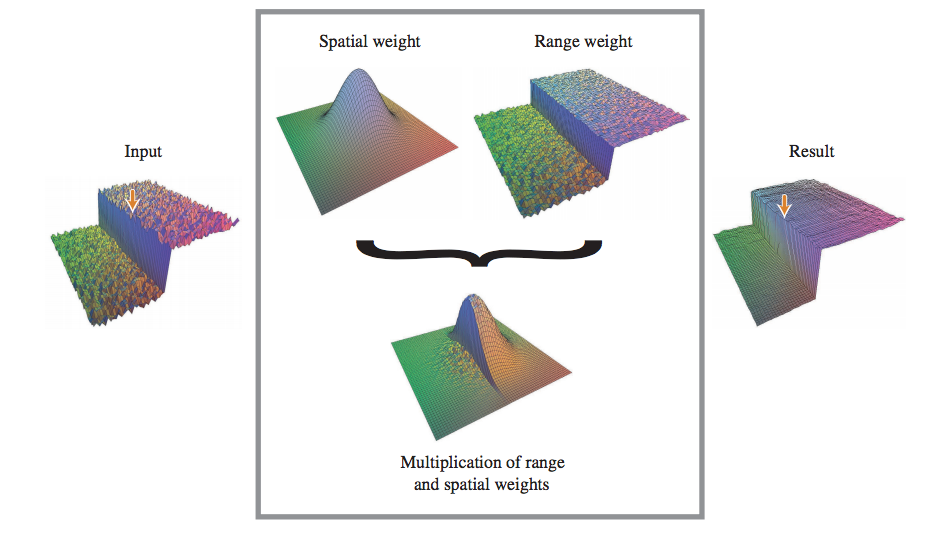
\includegraphics[scale=0.35]{OverallProcess}
\includegraphics[width=0.8\linewidth]{staircaseEffect}
\caption{Staircase Effect}
\end{figure}
\end{frame}

\begin{frame}
\frametitle{Limitations}
\begin{figure}
%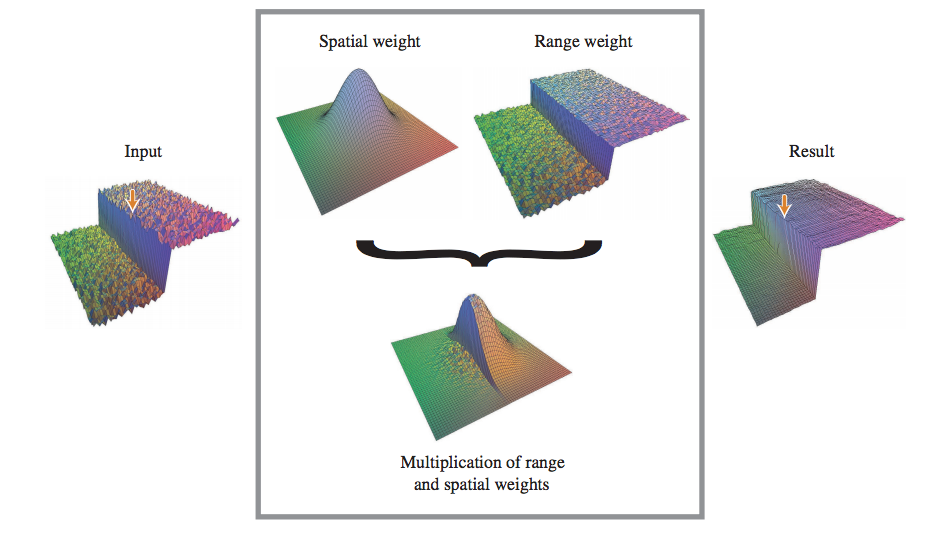
\includegraphics[scale=0.35]{OverallProcess}
\includegraphics[width=0.6\linewidth]{gradientReversal}
\caption{Gradient Reversal - False edges}
\end{figure}
\end{frame}

\section{Conclusions}


\begin{frame}
\frametitle{Conclusions}
\begin{itemize}
	\item Good for preserving edges
	\item CIE-Lab color space gives better output
	\item Parameters depend of domain filter depends on image properties
	\item Details are lost with large range values but edges not
	\item It's nonlinear
	\item Complexity - $O(n^{2})$
\end{itemize}
\end{frame}




















%------------------------------------------------

%\begin{frame}
%\frametitle{Blocks of Highlighted Text}
%\begin{block}{Block 1}
%Lorem ipsum dolor sit amet, consectetur adipiscing elit. Integer lectus nisl, ultricies in feugiat rutrum, porttitor sit amet augue. Aliquam ut tortor mauris. Sed volutpat ante purus, quis accumsan dolor.
%\end{block}
%
%\begin{block}{Block 2}
%Pellentesque sed tellus purus. Class aptent taciti sociosqu ad litora torquent per conubia nostra, per inceptos himenaeos. Vestibulum quis magna at risus dictum tempor eu vitae velit.
%\end{block}
%
%\begin{block}{Block 3}
%Suspendisse tincidunt sagittis gravida. Curabitur condimentum, enim sed venenatis rutrum, ipsum neque consectetur orci, sed blandit justo nisi ac lacus.
%\end{block}
%\end{frame}

%------------------------------------------------

%\begin{frame}
%\frametitle{Multiple Columns}
%\begin{columns}[c] % The "c" option specifies centered vertical alignment while the "t" option is used for top vertical alignment
%
%\column{.45\textwidth} % Left column and width
%\textbf{Heading}
%\begin{enumerate}
%\item Statement
%\item Explanation
%\item Example
%\end{enumerate}
%
%\column{.5\textwidth} % Right column and width
%Lorem ipsum dolor sit amet, consectetur adipiscing elit. Integer lectus nisl, ultricies in feugiat rutrum, porttitor sit amet augue. Aliquam ut tortor mauris. Sed volutpat ante purus, quis accumsan dolor.
%
%\end{columns}
%\end{frame}

%%------------------------------------------------
%\section{Second Section}
%%------------------------------------------------
%
%\begin{frame}
%\frametitle{Table}
%\begin{table}
%\begin{tabular}{l l l}
%\toprule
%\textbf{Treatments} & \textbf{Response 1} & \textbf{Response 2}\\
%\midrule
%Treatment 1 & 0.0003262 & 0.562 \\
%Treatment 2 & 0.0015681 & 0.910 \\
%Treatment 3 & 0.0009271 & 0.296 \\
%\bottomrule
%\end{tabular}
%\caption{Table caption}
%\end{table}
%\end{frame}
%
%%------------------------------------------------
%
%\begin{frame}
%\frametitle{Theorem}
%\begin{theorem}[Mass--energy equivalence]
%$E = mc^2$
%\end{theorem}
%\end{frame}
%
%%------------------------------------------------
%
%\begin{frame}[fragile] % Need to use the fragile option when verbatim is used in the slide
%\frametitle{Verbatim}
%\begin{example}[Theorem Slide Code]
%\begin{verbatim}
%\begin{frame}
%\frametitle{Theorem}
%\begin{theorem}[Mass--energy equivalence]
%$E = mc^2$
%\end{theorem}
%\end{frame}\end{verbatim}
%\end{example}
%\end{frame}
%
%%------------------------------------------------
%
%\begin{frame}
%\frametitle{Figure}
%Uncomment the code on this slide to include your own image from the same directory as the template .TeX file.
%\begin{figure}
%\includegraphics[width=0.8\linewidth]{overall}
%\end{figure}
%\end{frame}
%
%%------------------------------------------------
%
%\begin{frame}[fragile] % Need to use the fragile option when verbatim is used in the slide
%\frametitle{Citation}
%An example of the \verb|\cite| command to cite within the presentation:\\~
%
%This statement requires citation \cite{p1}.
%\end{frame}

%------------------------------------------------


%\setbeamertemplate{bibliography entry title}{}
%\setbeamertemplate{bibliography entry location}{}
%\setbeamertemplate{bibliography entry note}{}
%\begin{frame}[allowframebreaks]
%        \frametitle{References}
%        \bibliographystyle{amsalpha}
%        \bibliography{Report.bib}
%\end{frame}

%\begin{frame}%[t, allowframebreaks]
% \frametitle{References}
%\nocite{*}
%\bibliographystyle{plain}
%\bibliography{report}
% \end{frame}
%







\begin{frame}
\frametitle{References}
\footnotesize{
\begin{thebibliography}{99} % Beamer does not support BibTeX so references must be inserted manually as below

\bibitem[Wikipedia, 2015]{p1} Wikipedia (2015)
\newblock Bilateral filter

\bibitem[Tomasi, Manduchi, 2012]{p1} C. Tomasi, R. Manduchi  (1998)
\newblock Bilateral Filtering for Gray and Color Images
\newblock \emph{ICCV 1998}

\end{thebibliography}
}


\end{frame}

%------------------------------------------------

\begin{frame}
\Huge{\centerline{Thank you}}
\end{frame}

%----------------------------------------------------------------------------------------

\end{document} 